\section{Evaluation}\label{sec:Evaluation}
%Describe the evaluation set up briefly.

% 3 Graph that compares the precision/recall (F1) and time performance of our multiple approaches.


% Our approaches are: 
% 1. Graphs for 2D CNN with simple linear projection on one of the axis.
% 2. 2D CNN with improved transformation from 3D to 2D CNN
% 3. 2D CNN - with - separation and projection and then segmentation with DBSCAN 
% 4. 3D CNN
% 5. Different No. of Layers up to 3 and 2 different size of filter. 


% - We should run it on a standard machine (better on EC2 because it is better reproducible) and show the processing time performance. 


% - We present on our plots, Precision/Recall and Processing time. 





\begin{figure*}[!h]
\centering
\begin{minipage}{0.45\textwidth}
  \centering
        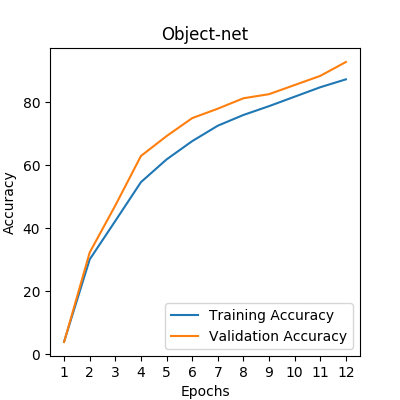
\includegraphics[width=1\linewidth]{images/accuracy.png}
        \caption{Training and Validation Accuracy}
        \label{fig:ground_before}
\end{minipage}%
\begin{minipage}{0.45\textwidth}
  \centering
        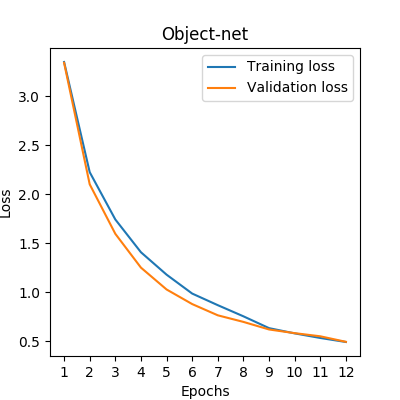
\includegraphics[width=1\linewidth]{images/loss.png}
        \caption{Training and Validation Loss}
        \label{fig:after}
\end{minipage}%
% \caption{General caption.} \label{fig:1}
\end{figure*}








